\documentclass{article}

\usepackage{fancyhdr}
\usepackage{extramarks}
\usepackage{amsmath}
\usepackage{amsthm}
\usepackage{amsfonts}
\usepackage{tikz}
\usepackage[plain]{algorithm}
\usepackage{algpseudocode}
\usepackage{graphicx}
\usetikzlibrary{automata,positioning}
\usepackage{pdfpages,float}

%
% Basic Document Settings
%

\topmargin=-0.45in
\evensidemargin=0in
\oddsidemargin=0in
\textwidth=6.5in
\textheight=9.0in
\headsep=0.25in

\linespread{1.1}

\pagestyle{fancy}
\lhead{\hmwkAuthorName}
\chead{\hmwkClass\ (\hmwkClassInstructor\ \hmwkClassTime): \hmwkTitle}
\rhead{\firstxmark}
\lfoot{\lastxmark}
\cfoot{\thepage}

\renewcommand\headrulewidth{0.4pt}
\renewcommand\footrulewidth{0.4pt}

\setlength\parindent{0pt}

%
% Create Problem Sections
%

\newcommand{\enterProblemHeader}[1]{
    \nobreak\extramarks{}{Problem \arabic{#1} continued on next page\ldots}\nobreak{}
    \nobreak\extramarks{Problem \arabic{#1} (continued)}{Problem \arabic{#1} continued on next page\ldots}\nobreak{}
}

\newcommand{\exitProblemHeader}[1]{
    \nobreak\extramarks{Problem \arabic{#1} (continued)}{Problem \arabic{#1} continued on next page\ldots}\nobreak{}
    \stepcounter{#1}
    \nobreak\extramarks{Problem \arabic{#1}}{}\nobreak{}
}

\setcounter{secnumdepth}{0}
\newcounter{partCounter}
\newcounter{homeworkProblemCounter}
\setcounter{homeworkProblemCounter}{1}
\nobreak\extramarks{Problem \arabic{homeworkProblemCounter}}{}\nobreak{}

%
% Homework Problem Environment
%
% This environment takes an optional argument. When given, it will adjust the
% problem counter. This is useful for when the problems given for your
% assignment aren't sequential. See the last 3 problems of this template for an
% example.
%
\newenvironment{homeworkProblem}[1][-1]{
    \ifnum#1>0
        \setcounter{homeworkProblemCounter}{#1}
    \fi
    \section{Problem \arabic{homeworkProblemCounter}}
    \setcounter{partCounter}{1}
    \enterProblemHeader{homeworkProblemCounter}
}{
    \exitProblemHeader{homeworkProblemCounter}
}

%
% Homework Details
%   - Title
%   - Due date
%   - Class
%   - Section/Time
%   - Instructor
%   - Author
%

\newcommand{\hmwkTitle}{Homework\ \#10}
\newcommand{\hmwkDueDate}{Nov 24, 2019}
\newcommand{\hmwkClass}{CMSE 820}
\newcommand{\hmwkClassTime}{}
\newcommand{\hmwkClassInstructor}{Professor Yuying Xie}
\newcommand{\hmwkAuthorName}{\textbf{Boyao Zhu}}

%
% Title Page
%

\title{
    \vspace{2in}
    \textmd{\textbf{\hmwkClass:\ \hmwkTitle}}\\
    \normalsize\vspace{0.1in}\small{Due\ on\ \hmwkDueDate\ at 11:59pm}\\
    \vspace{0.1in}\large{\textit{\hmwkClassInstructor\ \hmwkClassTime}}
    \vspace{3in}
}

\author{\hmwkAuthorName}
\date{}

\renewcommand{\part}[1]{\textbf{\large Part \Alph{partCounter}}\stepcounter{partCounter}\\}

%
% Various Helper Commands
%

% Useful for algorithms
\newcommand{\alg}[1]{\textsc{\bfseries \footnotesize #1}}

% For derivatives
\newcommand{\deriv}[1]{\frac{\mathrm{d}}{\mathrm{d}x} (#1)}

% For partial derivatives
\newcommand{\pderiv}[2]{\frac{\partial}{\partial #1} (#2)}

% Integral dx
\newcommand{\dx}{\mathrm{d}x}

% Alias for the Solution section header
\newcommand{\solution}{\textbf{\large Solution}}

% Probability commands: Expectation, Variance, Covariance, Bias
\newcommand{\E}{\mathrm{E}}
\newcommand{\Var}{\mathrm{Var}}
\newcommand{\Cov}{\mathrm{Cov}}
\newcommand{\Bias}{\mathrm{Bias}}

\begin{document}

\maketitle

\pagebreak

\begin{homeworkProblem}
\textbf{Solution}//
Define the local charts on \(S^2=\{(x,y,z) : x^2+y^2+z^2=1\}\) using: (1) polar coordinate representation; (2) stereographical projection.\\
\\
Let \(\Omega_1 = S^2 \setminus \{0,0,1\}\) and \(\Omega_2 = S^2 \setminus \{0,0,-1\}\) be two open sets in \(\mathbb{R}\).  Then \(C = \{\Omega_i : i\in\{1,2\}\}\) is an open cover of \(S^2\).\\
Applying stereographical projection for these two open sets, we can define the following mappings
\[
\begin{split}
\phi_1 : \Omega_1 \rightarrow \mathbb{R}^2, \phi_1(x,y,z) & = \left( \frac{x}{1-z}, \frac{y}{1-z}\right)\\
\phi_1^{-1} : \mathbb{R}^2 \rightarrow \Omega_1, \phi_1^{-1}(X,Y) & = \left( \frac{2X}{1+X^2+Y^2},\frac{2Y}{1+X^2+Y^2},\frac{-1+X^2+Y^2}{1+X^2+Y^2}\right)\\
\phi_2 : \Omega_2 \rightarrow \mathbb{R}^2, \phi_2(x,y,z) & = \left( \frac{x}{1+z}, \frac{y}{1+z}\right)\\
\phi_2^{-1} : \mathbb{R}^2 \rightarrow \Omega_2, \phi_1^{-1}(X,Y) & = \left( \frac{2X}{1+X^2+Y^2},\frac{2Y}{1+X^2+Y^2},\frac{1-X^2-Y^2}{1+X^2+Y^2}\right)
\end{split}
\]
It is easy to check that \(\phi_1\) and \(\phi_2\) are homeomorphisms, so they are two local charts under the stereographical projection that form an atlas of \(S^2\).\\
Rewriting the Cartesian coordinate representation of \(S^2\) in the polar coordinate representation, we have a different set of local charts.
\[
\begin{split}
\psi_1 : \Omega_1 \rightarrow [0,\infty) \times [0,2\pi), \psi_1(x,y,z) &= \left(\frac{\sqrt{x^2+y^2}}{1-z}, \text{arccos}\frac{y}{x}\right)\\
\psi_1^{-1} :  [0,\infty) \times [0,2\pi) \rightarrow \Omega_1, \psi_1^{-1}(r,\theta) &= \left(\frac{2r\text{cos}\theta}{1+r^2}, \frac{2r\text{sin}\theta}{1+r^2},\frac{r^2-1}{1+r^2}\right)\\
\psi_2 : \Omega_2 \rightarrow [0,\infty) \times [0,2\pi), \psi_2(x,y,z) &= \left(\frac{\sqrt{x^2+y^2}}{1+z}, \text{arccos}\frac{y}{x}\right)\\
\psi_2^{-1} :  [0,\infty) \times [0,2\pi) \rightarrow \Omega_2, \psi_2^{-1}(r,\theta) &= \left(\frac{2r\text{cos}\theta}{1+r^2}, \frac{2r\text{sin}\theta}{1+r^2},\frac{-r^2+1}{1+r^2}\right)
\end{split}
\]

\end{homeworkProblem}


\begin{homeworkProblem}
\textbf{Solution}\\

Kernel PCA is only able to separate the data points into 3 rays of similar color, which still differs quite a great deal from the original data. LLE, on the other hand, is capable of “unrolling” the data, restoring the 2D-manifold features (almost perfectly). When the high-dimensional data resembles some low-dimensional manifold embedded in the high- dimensional space, LLE outperforms plain kernel PCA.


\begin{figure}[H]
	\centerline{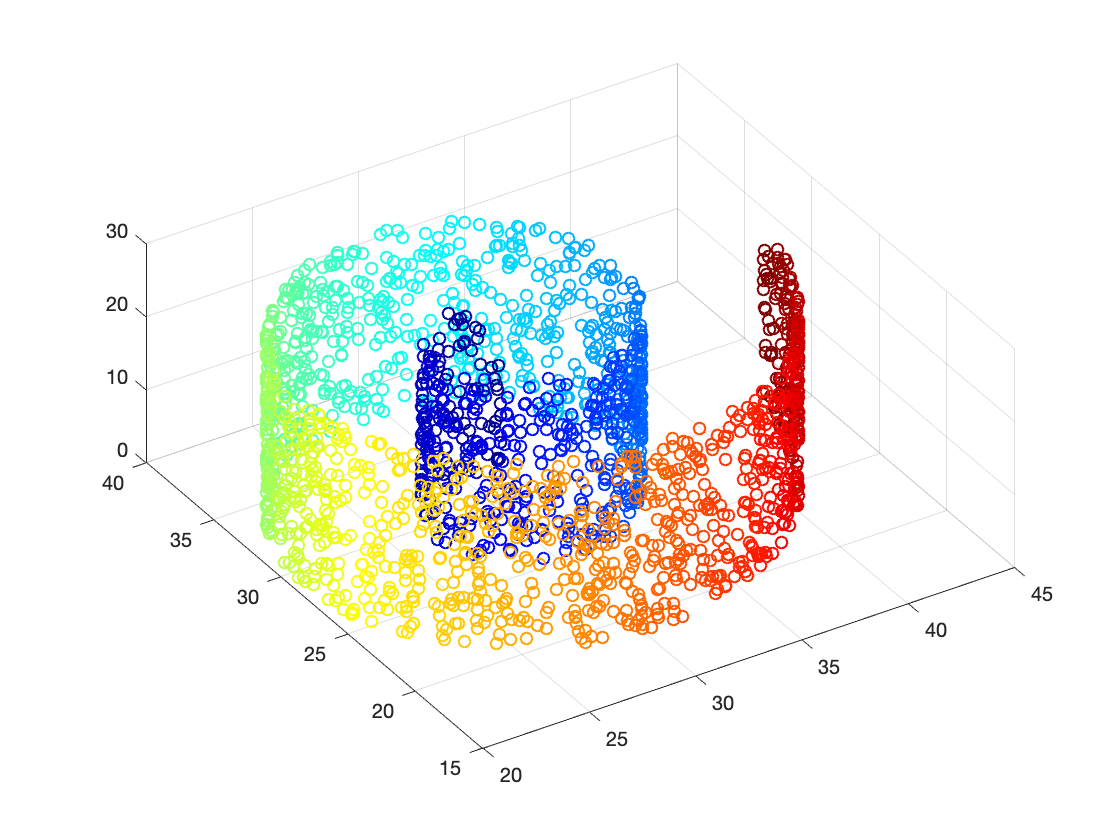
\includegraphics[scale=0.3]{1.png}}
	\caption{Original data in 3D}
\end{figure}


\begin{figure}[H]
	\centerline{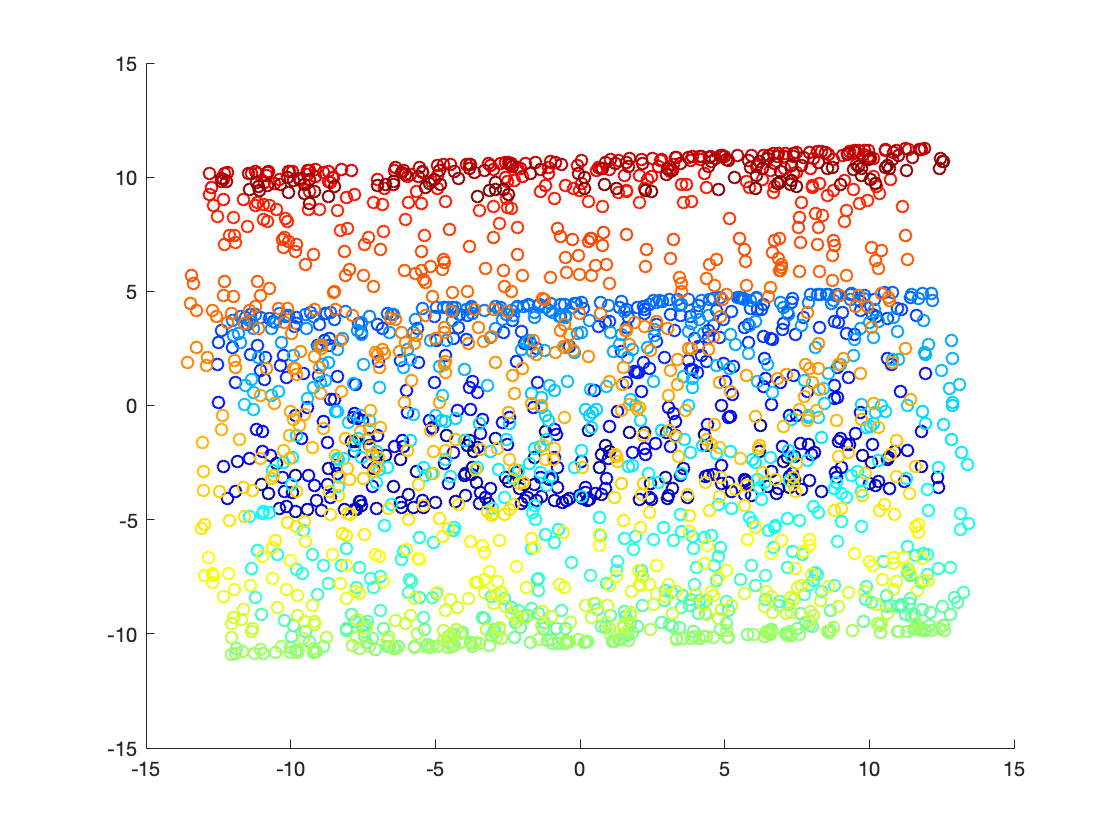
\includegraphics[scale=0.3]{2.png}}
	\caption{By PCA, Data projected onto the top 2 PCs}
\end{figure}

\begin{figure}[H]
	\centerline{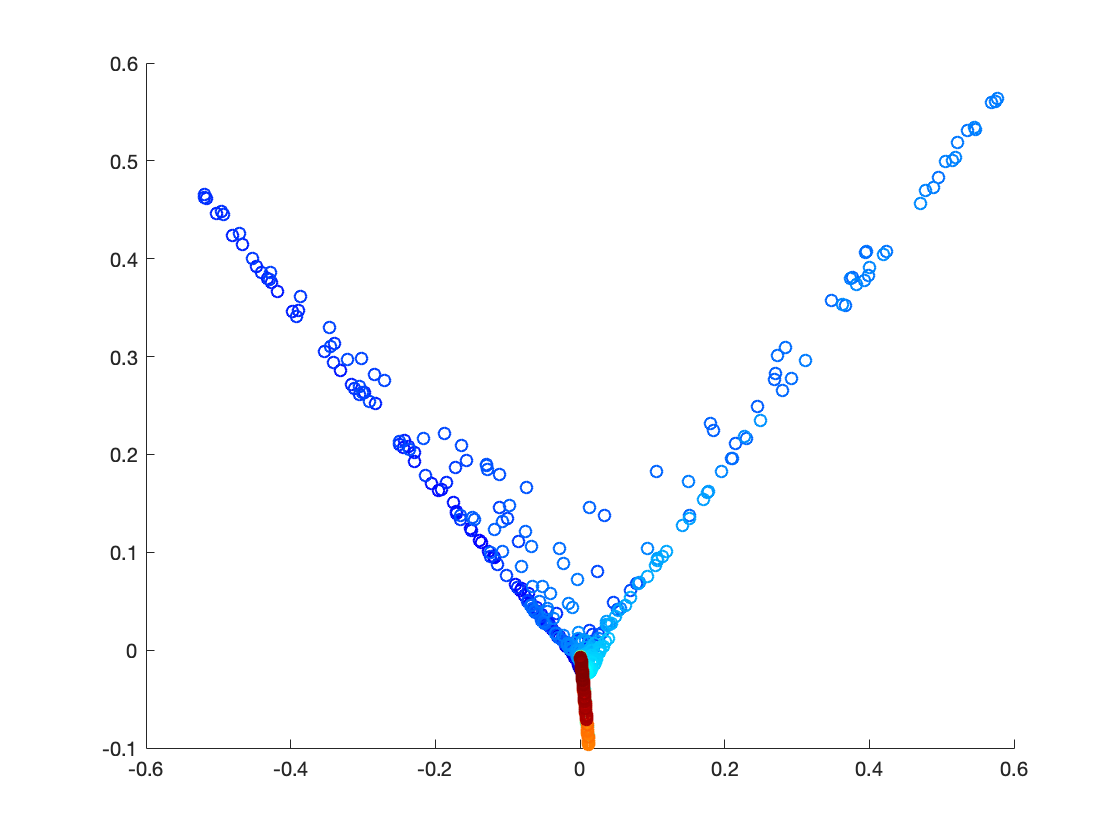
\includegraphics[scale=0.3]{3.png}}
	\caption{By Kernel PCA, Data projected on the top 2 PCs}
\end{figure}

\begin{figure}[H]
	\centerline{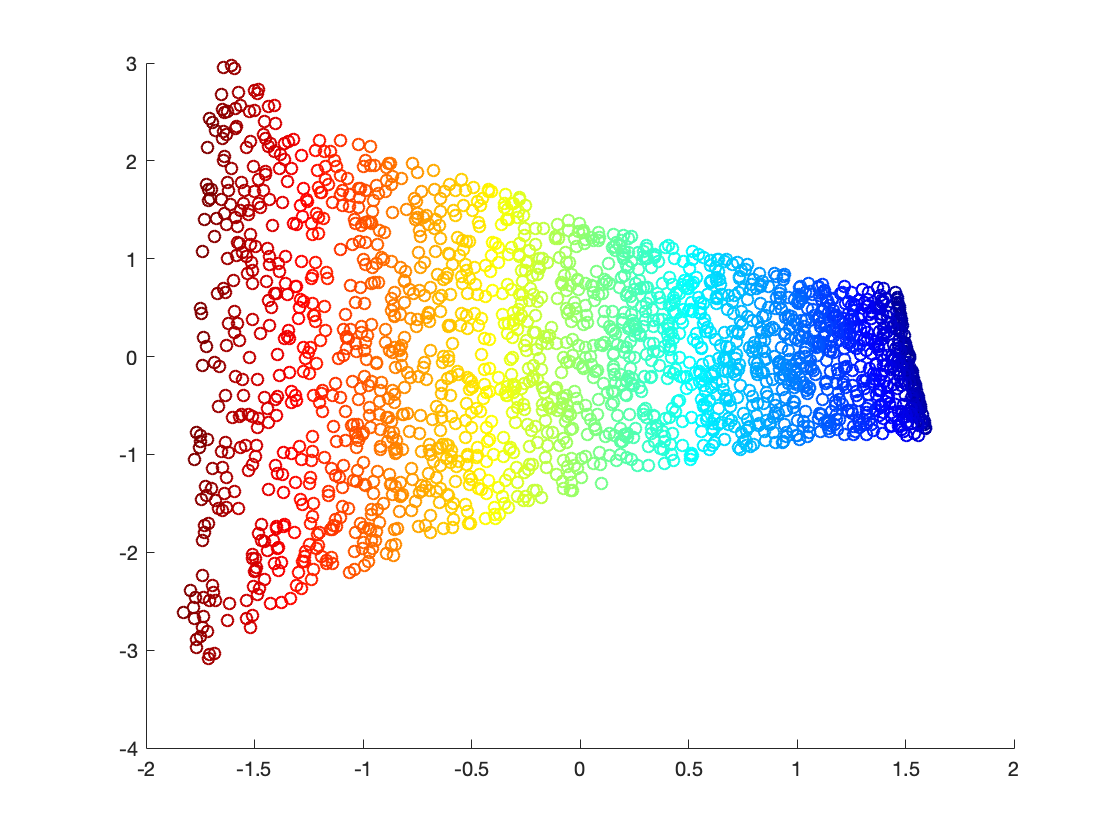
\includegraphics[scale=0.3]{4.png}}
	\caption{LLE with 12-nearest neighbors, Data reduced to 2D}
\end{figure}


\end{homeworkProblem}



\begin{homeworkProblem}
\textbf{Solution}\\
Laplacian Eigenmaps (LE).\\
Let \(x_1,\cdot\cdot\cdot, x_n\in\mathbb{R}^p\) be the high dimensional data points.  For any fixed scalar \(\epsilon>0, x_i \text{ and } x_j\) are called \(\epsilon\)-neighbors of each other if and only if \(\lVert x_i-x_j\rVert_2\leq \epsilon\).  Fix another scalar \(\sigma^2>0\), and we can define a weight \(w_{ij} = \text{exp}(-\frac{\lVert x_i-x_j\rVert_2^2}{\sigma^2})\) if \(x_i\) and \(x_j\) are \(\epsilon\)-neighbors and \(w_{ij}=0\) otherwise.  A reasonable low dimensional embedding \(y_1, \cdot\cdot\cdot, y_n\) minimizes the following objective function
\[
\sum_{i,j}w_{ij}\lVert y_i-y_j\rVert_2^2.
\]

\textbf{3.1 a}\\
Prove that min\(\frac{1}{2}\sum w_{ij}\lVert y_i-y_j\rVert_2^2=\text{min}Tr(YLY^T\), where \(Y=[y_1, \cdot\cdot\cdot, y_n]\) and \(L=D-A\) with \(A_{ij}=w_{ij}\) and \(D\) being a diagonal matrix with \(D_{ii}=\Sigma_j w_{ij}\).  The matrix \(L\) is called graph laplacian.\\
\textbf{Proof}: Starting from the summation, we have
\[
\begin{split}
\frac{1}{2}\sum_{ij}w_{ij}\lVert y_i-y_j\rVert_2^2 &= \frac{1}{2}\sum_{ij}w_{ij}(y_i^Ty_i-y_i^Ty_j-y_j^Ty_i+y_j^Ty_j)\\
&= \frac{1}{2}[2\sum_i(\sum_j w_{ij})y_i^Ty_i-2\sum_{ij}w_{ij}y_i^Ty_j]\\
&= \sum_i(\sum_j w_{ij})y_i^Ty_i - \sum_{ij}w_{ij}y_i^Ty_j
\end{split}
\]

Starting from the trace, we have
\[
\begin{split}
\text{Tr}(YLY^T) &= \sum_i(YLY^T)_{ii}\\
&= \sum_i[\sum_{jk}Y_{ij}L_{jk}(Y^T)_{ki}]\\
&= \sum_i(\sum_{jk}Y_{ij}L_{jk}Y_{ik})\\
&= \sum_{jk} L_{jk}(\sum_i Y_{ij}Y_{ki}\\
&= \sum_{jk} L_{jk}y_j^Ty_k\\
&= \sum_{ij}(D_{ij}-A_{ij})y_i^Ty_j\\
&= \sum_{ij}(\sum_k w_{ik})\delta_{ij}y_i^Ty_j - \sum_{ij}w_{ij}y_i^Ty_j\\
&= \sum_i(\sum_j w_{ij})y_i^Ty_i - \sum_{ij}w_{ij}y_i^Ty_j\\
&= \frac{1}{2}\sum_{ij}w_{ij}\lVert y_i-y_j\rVert_2^2
\end{split}
\]

\textbf{3.2 b}\\
\[
\hat{Y}=\underset{Y}{\text{arg min}}\text{Tr}(YLY^T) \text{ subject to } YDY^T = I \text{ and } YD\textbf{1} = 0
\]
Show that the solution \(\hat{Y}\in\mathbb{R}^{d\times n}\) are given by the eigenvectors corresponding to the lowest \(d\) eigenvalues of the generalized eigenvalue problem
\[
Ly = \lambda Dy
\]
\textbf{Proof}: We ignore the constraint \(YD\textbf{1}= 0\) for the time being and write down the Lagrangian
\[
L(Y,\Lambda) = \text{Tr}(YLY^T)+\langle \Lambda, I-YDY^T\rangle
\]
where \(\Lambda\) is the symmetric Lagrangian matrix coefficients, because \(YDY^T\) is symmetric.  Taking the derivative respect to \(Y\), we have
\[
\frac{\partial L}{\partial Y} = 2(LY^T-\Lambda DY^T)
\]
Setting the derivative to be 0 and rewriting \(\Lambda = U\Sigma U^T\) in terms of its eigenvalue decomposition with \(\Sigma\) beging diagonal and \(U\) being orthogonal,
\[
LY^T -\Lambda DY^T = LY^T-U\Sigma U^TDY^T = LY^T-U\Sigma DU^TY^T = 0 \Longrightarrow LY'=DY'\Sigma \quad (\ast)
\]
where \(Y' = (UY)^T\) and we have used the fact that matrix multiplication with any diagonal matrix is commutative.\\
Note that for any \(Y\) and any orthogonal matrix \(O\), \(\text{Tr}(YLY^T)=\text{Tr}((OY)L(OY)^T)\).  \(\hat{Y}\) can be determined at most up to rotations.  This suggests that we should solve the generalized eigenvalue problem
\[
Ly = \lambda Dy \quad (\ast\ast)
\]
Furthermore, we should show that for any \(y^{\ast}\) satistfying equation \((\ast\ast)\), \(\textbf{1}^TDy^{\ast}=0\)
\[
\begin{split}
& \textbf{1}^TDy^{\ast} =\textbf{1}^T\frac{1}{\lambda}Ly = 0\\
\Longleftarrow\quad & \textbf{1}^TL = 0^T\\
\Longleftarrow\quad & \forall j, \sum_j L_{ij} = \sum_j D_{ij}-A_{ij} = D_{ii} - \sum_j W_{ij} = \sum_j W_{ij} - \sum_j W_{ij} = 0 
\end{split}
\]
So we can let \(\hat{Y} = [y_1, \cdot\cdot\cdot, y_d]^T\) such that \(y_1, \cdot\cdot\cdot, y_d\) are solutions to the generalized eigenvalue problem corresponding to the smallest eigenvalues.  It is clear that \(\hat{Y}D\hat{Y}^T = I\) and \(\hat{Y}D\textbf{1}=0\)
\end{homeworkProblem}



\begin{homeworkProblem}
\textbf{Solution}\\
In the derivation of LLE, we define 
\[
M = (I_N-W)^T(I_N-W)
\]
Prove that \(M\textbf{1} = 0\)\\
\textbf{Proof} Recall that
\[
\forall i, \sum_j W_{ij} = W_i, \textbf{1} = 1
\]
It follows that
\[
W\textbf{1} = \textbf{1}
\]
Hence,
\[
M\textbf{1} = (I_N-W)^T(I_N-W)\textbf{1} = (I_N-W)^T(\textbf{1}-\textbf{1}) =0
\]

\end{homeworkProblem}



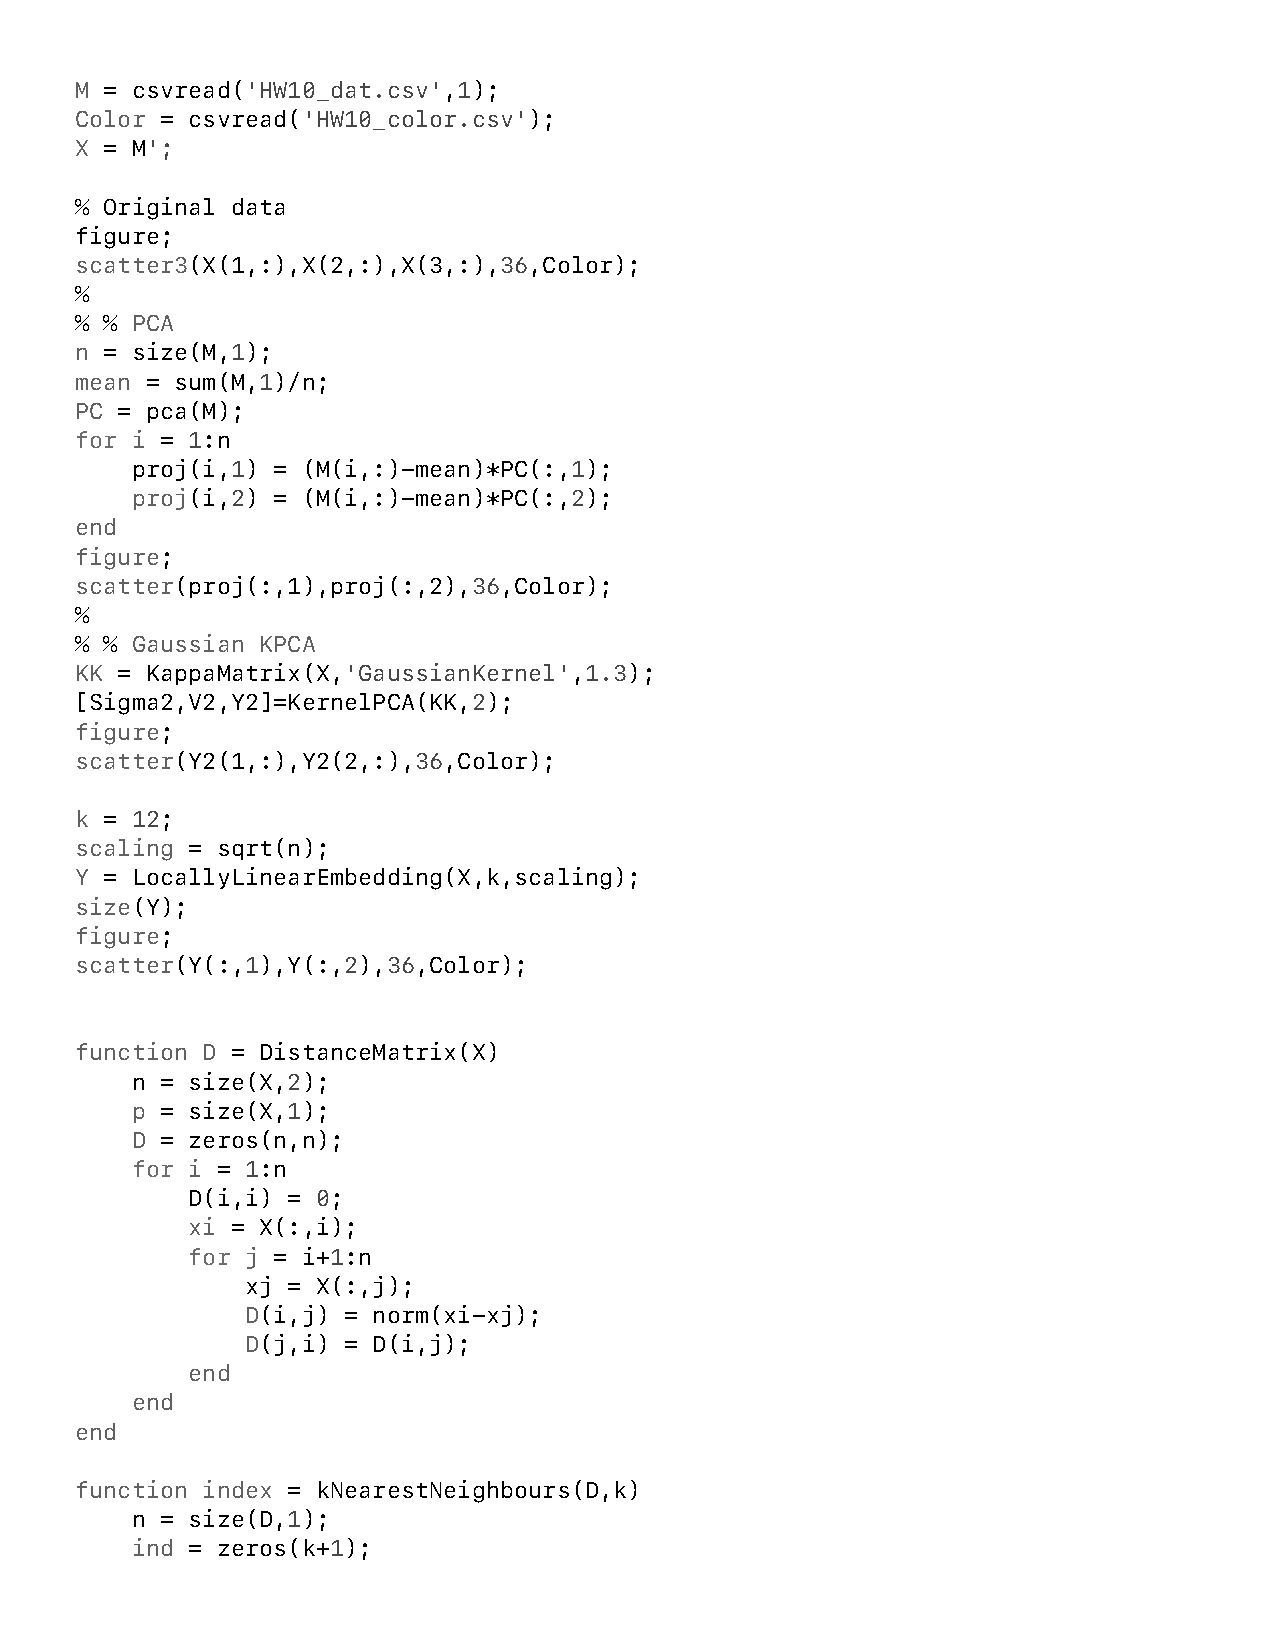
\includepdf[page={-}]{HW10_code.pdf}











\end{document}